\documentclass[border=10pt]{standalone}

\usepackage{tikz}
\usepackage{tikzsymbols}
\usetikzlibrary{calc,patterns,shapes.geometric}

\def\centerarc[#1](#2)(#3:#4:#5){\draw[#1] ($(#2)+({#5*cos(#3)},{#5*sin(#3)})$) arc (#3:#4:#5);}

\begin{document}
	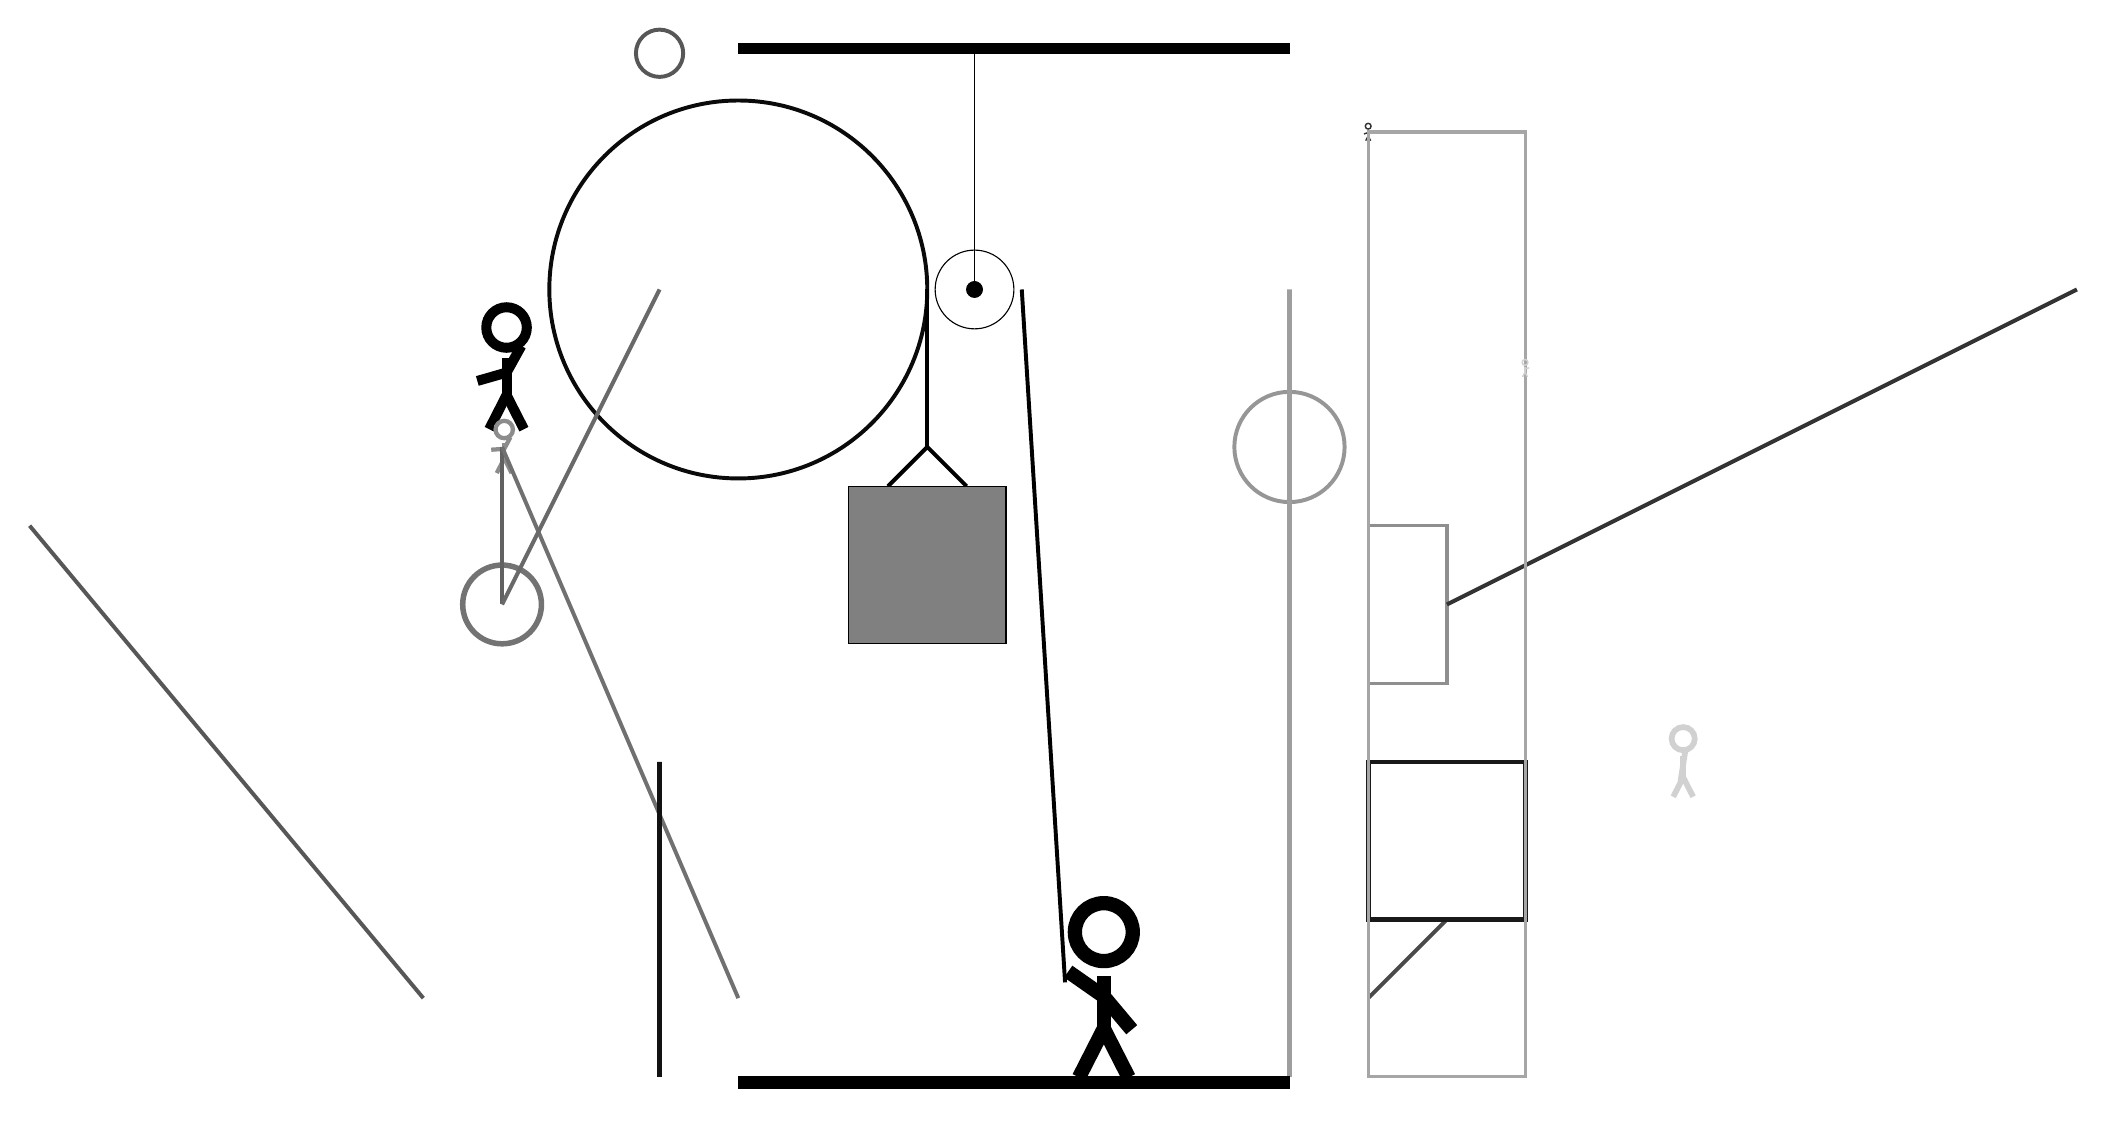
\begin{tikzpicture}
		%%%%% START %%%%%
		
		\draw[fill=black] (-2, 10) rectangle (5, 10.125);
		
		\node[line width=0.4mm, color=black!100] at (-5, 6) {\Strichmaxerl[7][16][61]};
		
		\draw [line width=0.7mm, color=black!55](-5, 3) circle (0.5);
		\draw [line width=0.5mm, color=black!66](-3, 10) circle (0.3);
		\draw[line width=0.4mm, color=black!44] (6, 4) rectangle (7, 2);
		\draw[line width=0.5mm, color=black!71](7, -1) -- (6, -2);
		\node[line width=0.6mm, color=black!45] at (-5, 5) {\Strichmaxerl[3][4][62]};
		
		\draw[line width=0.5mm, color=black!62](-5, 5) -- (-5, 3);
		\node[line width=0.3mm, color=black!18] at (10, 1) {\Strichmaxerl[4][81][81]};
		\draw [line width=0.5mm, color=black!41](5, 5) circle (0.7);
		\draw[line width=0.5mm, color=black!56](-5, 5) -- (-2, -2);
		\draw [line width=0.5mm, color=black!96](-2, 7) circle (2.4);
		\draw[line width=0.7mm, color=black!38] (5, -3) rectangle (5, 7);
		\draw[line width=0.7mm, color=black!93] (-3, -3) rectangle (-3, 1);
		\node[line width=0.6mm, color=black!80] at (6, 9) {\Strichmaxerl[1][17][14]};
		\draw[line width=0.5mm, color=black!80](7, 3) -- (15, 7);
		\draw[line width=0.5mm, color=black!66](-6, -2) -- (-11, 4);
		\draw[line width=0.6mm, color=black!90] (6, -1) rectangle (8, 1);
		\draw[line width=0.5mm, color=black!59](-3, 7) -- (-5, 3);
		\draw[line width=0.4mm, color=black!35] (6, -3) rectangle (8, 9);
		\node[line width=0.2mm, color=black!18] at (8, 6) {\Strichmaxerl[1][89][14]};
		
		\draw (1, 7) circle (0.5);
		\draw[fill=black] (1, 7) circle (0.1);
		\draw (1, 10) -- (1, 7);
		
		\draw[line width=0.5mm] (-0.1, 4.5) -- (0.4, 5.0) -- (0.9, 4.5);
		\draw[fill=black!50] (-0.6, 4.5) rectangle (1.4, 2.5);
		
		\draw[line width=0.5mm] (0.4, 7) -- (0.4, 5.0);
		\centerarc[line width=0.5mm](1, 7)(0:180:0.6);
		\draw[line width=0.5mm](1.6, 7) -- (2.15, -1.8);
		
		\node at (2.6, -1.9) {\Strichmaxerl[10][-35][-50]};
		
		\draw[fill=black] (-2, -3) rectangle (5, -3.15);
		
		%%%%% END %%%%%
	\end{tikzpicture}
\end{document}